\chapter{Konstruktion des Skripts}
\label{cha:konstruktion}

Dieses Kapitel behandelt die Erstellung der Tilesets, die zur Simulation des zuvor erörterten Konzepts mit der Simulationsumgebung NetTAS benötigt werden. Im Zentrum dieses Kapitels steht ein Python-Skript, das im Rahmen dieser Arbeit entwickelt wurde. Das Skript, seine Funktionen und Eigenschaften werden im Folgenden detailiert beschrieben. Interessierte können das Skript über den QR-Code am Seitenrand \marginnote{\qrcode[height=1cm]{https://github.com/Falkenheim/Tile-Generator}} oder über die Links im Anhang~\ref{app:code} auf Github einsehen. Zunächst wird die Simulationsumgebung NetTAS erläutert. Im Folgenden wird dargelegt, wie das Skript anhand verschiedener Parameter Tilesets erstellt. Für die generierten Tilesets wird zudem eine Erweiterung vorgestellt, di Prüfsummen auf Tilesets implementiert. Es wird auch erörtert, welche Voraussetzungen für externe Tilesets bestehen, damit sie durch das Skript korrekt modifiziert werden können. Hierzu wird ein Farbcode eingeführt. Zudem wird das grafische Interface des Skripts beleuchtet. Das Kapitel endet mit einer Beschreibung des Gesamtablaufs des Skripts, einschließlich der Umsetzung von Flags, Prioritätstiles und Snaked-Proofreading auf beliebigen Tilesets.

\section{NetTAS}

Um die Konstruktion von den im vorherigen Kapitel vorgestellten Anforderungen durchführen zu können, muss zunächst auf die Simulationsumgebung NetTAS und den Aufbau von Tiles und Tilesets in diesem Kontext eingegangen werden.

Die in Kapitel \ref{cha:grundlagen} vorgestellten Tile-Assembly-Modelle können in der Simulationsumgebung \emph{NetTAS} verwendet werden, um Tilesets zu simulieren. Dabei handelt es sich um die Tile-Assembly-Modelle aTAM, kTAM, 2HAM und kTHAM. Das Tool wurde in TypeScript programmiert und kann über eine Webanwendung über den Browser verwendet werden \cite{kaussow2022thesis}. Dieses Tool wird nicht nur wegen der besseren Verfügbarkeit und Dokumentation für die Arbeit verwendet, sondern auch, weil es die einzige Simulationsumgebung ist, die das kTHAM beinhaltet.

In NetTAS können Tilesets erstellt werden, indem Label, Kleberbezeichner und Kleberstärken in einem grafischen Interface eingegeben werden. Diese Tilesets können in JSON-Dateien gespeichert und geladen werden. Die JSON-Dateien haben eine spezifische Form, die in der Konstruktion des Skripts einen entscheidenden Faktor spielt. 

Dafür wird zunächst die Form eines Tilesets in JSON vorgestellt und analysiert:
\newpage
\begin{lstlisting}[caption={[Darstellung des Tilesets in einer JSON-Datei]{Darstellung eines beispielhaften Tilesets in JSON-Form. Tiles werden in \texttt{\_tiles} gelistet. Hier ist ein weißes Tile mit dem Bezeichner \texttt{A} und den folgenden Klebern dargestellt: nördlicher Kleber \texttt{a} der Stärke eins, östlicher Kleber \texttt{b} mit Stärke zwei, südlicher Kleber \texttt{c} mit Stärke zwei und keinem Kleber oder Label auf der westlichen Seite des Tiles. Auch wird ein Tile \texttt{B} angedeutet, um zu zeigen, wie weitere Tiles aufgelistet werden.}}, label=lst:tileset_json]
{
    "_tiles": [
        {
            "label": "A",
            "glues": [
                {
                    "label": "a",
                    "strength": 1
                },
                {
                    "label": "b",
                    "strength": 2
                },
                {
                    "label": "c",
                    "strength": 2
                },
                {
                    "label": "",
                    "strength": 0
                }
            ],
            "color": "white"
        },
        {
            "label": "B",
                .
                .
                .
        }
    ]
}
\end{lstlisting}

Jedes Tile des Tilesets wird in den \emph{\_tiles} gespeichert. Ein Tile enthält den Bezeichner \emph{label} und die zugehörigen Kleber \emph{glues}. Letztere bestehen aus vier Tupeln, wobei jedes Tupel den Kleberbezeichner \emph{label} und die Kleberstärke \emph{strength} für eine bestimmte Seite des Tiles repräsentiert. Dabei ist die Reihenfolge wie folgt festgelegt:
\begin{enumerate}
    \item Tupel: nördlicher Kleber (hier Bezeichner \texttt{a}, mit Stärke eins)
    \item Tupel: östlicher Kleber (hier Bezeichner \texttt{b}, mit Stärke zwei)
    \item Tupel: südlicher Kleber (hier Bezeichner \texttt{c}, mit Stärke zwei)
    \item Tupel: westlicher Kleber (hier Bezeichner \verb|""|, mit Stärke null)
\end{enumerate}
Die letzte Information ist die Farbe des Tiles. Diese wird in der Variable \emph{color} gespeichert. Durch Aneinanderreihung solcher Tiles kann so ein Tileset mit allen benötigten Informationen gespeichert oder geladen werden.

\section{Die Generierung von Tilesets im Skript}

Diese vorgestellte Struktur kann in einem Python-Skript nachgebaut werden. So können Tilesets verändert, beziehungsweise generiert werden. Bei der Generierung eines Tilesets wird im Skript auf die Nachrichtencodierung aus dem letzten Kapitel geachtet. Für eine Anzahl an Nachrichten in einem fiktiven System mit Gewichtungen für Tileset- und Assemblygröße, wird ein Tileset automatisch generiert. Diese Codierung hält sich dabei an den Ansatz, bei welchem die Information in die Tilebezeichner codiert werden kann. So besitzt jedes generierte Tileset bei der Self-Assembly eine Molekülhöhe von eins. Der Vorgang für die Generierung des Tileset kann durch folgenden Pseudocode dargestellt werden:
\begin{lstlisting}[language=python, caption={[Pseudocode für die Generierung eines Tilesets]{Pseudocode für die Generierung eines Tilesets für gegebene Anzahl zu kodierenden Nachrichten und den Gewichtungen von Tileset- und Assemblygröße. Es wird die optimale Basis für die Anzahl der Nachrichten nach den gegebenen Gewichtungen berechnet. Anschließend werden aus der Anzahl und der Basis die erforderlichen Ziffern ermittelt. Mit beiden Parametern kann das Tileset generiert werden.}}, label=lst:generate]
# mc = message count 
# tw = tileset weight 
# aw = assembly weight
def generate_data(mc, tw, aw):
    base = find_best_base(mc, tw, aw)
    digits = get_digits_for(mc, base)
    tiles = []
    tiles.append(generate_seedtile())
    for each digit in digits:
        for each number in base:
            tiles.append(generate_tile(digit, number))
    tile.append(generate_ligand())    
    return {"_tiles": tiles}
\end{lstlisting}
Zur Generierung des optimalen Tilesets, wird zuerst die optimale Basis mit der Funktion \texttt{find\_best\_base} bestimmt. Nachdem diese Basis festgelegt wurde, lässt sich ermitteln, wie viele Ziffern codiert werden müssen. Sobald die optimale Basis und die Anzahl der Ziffern durch die Variablen \texttt{base} und \texttt{digits} festgelegt sind, kann das Tileset generiert werden. Zunächst wird die Seed-Assembly generiert. Danach kann für jede Ziffernstelle und jede Zahl in der Basis ein Tile erstellt werden. Dabei wird die Zahl im Tilebezeichner notiert, die Kleberbezeichner legen die Stelle in der Ziffernfolge fest. Zuletzt wird der Ligand erstellt, der sich an die letzte Ziffernstelle binden kann. 

\section{Die Generierung von Prüfsummen in Nanonetzwerken}

Eine Erweiterung zur Generierung von Tilesets, ist die Generierung von Tilesets mit integrierter Prüfsumme. Dabei wird die gleiche Idee verwendet, jedoch wird sie rekursiv durchgeführt. Folgender Pseudocode stellt die Idee zur Generierung von Tilesets mit Prüfsummen dar:

\begin{lstlisting}[language=python, caption={[Pseudocode für die Generierung eines Tilesets mit Prüfsumme]{Pseudocode für die Generierung eines Tilesets mit Prüfsumme. Die Rekursion wird dabei dazu genutzt, um exponentiell mehr Tiles für jede weitere Ziffernstelle zu erstellen. Auch muss statt einem einzelnen letzten Tile, wie in \texttt{generate\_tile}, für alle codierten Nachrichten ein Prüfsummentile erstellt werden.}}, label=lst:generate_checksum]
# mc = message count  
# tw = tileset weight
# aw = assembly weight
def generate_data_with_checksum(mc, tw, aw):
    base = find_best_base(mc, tw, aw)
    digits = get_digits_for(mc, base)
    tiles = []
    tiles.append(generate_seedtile())
    for each digit:
        tiles.append(generate_data_recursive(digit, base))
    for each num in message_count:
        tiles.append(generate_checksumligand())

def generate_data_recursive(digit, base):
    temp_tiles = []
    if digit == 1:
        for each num in base
            temp_tiles.append(generate_tile())
    else:
        temp_tiles.extend(generate_data_recursive(digit-1))
\end{lstlisting}
Durch die Konstruktion mit Prüfsumme ist das Tileset in den meisten Fällen sehr groß. Deshalb wurde im Skript und in dieser Arbeit darauf verzichtet, die Prüfsummengenerierung für andere Tilesets und Moleküle zu implementieren. Diese wären jedoch analog, wobei weitere Informationen gesammelt werden müssen. Dabei muss jedes Tileset auf Positionen aller Tiles in der Self-Assembly analysiert werden. Dann kann festgestellt werden, wie viele Tiles an welchen Stellen des Moleküls vorkommen können. Daraus kann durch das gleiche Prinzip wie im Code~\ref{lst:generate_checksum} das Tileset mit einer Prüfsumme versehen werden.

\section{Farbcode als Anforderung an Tilesets}

Nachdem nun die Generierung von Tilesets durch das Skript detailliert erläutert wurde, sollen im Weiteren die Anforderungen für die korrekte Anwendung der Mechanismen im Skript beschrieben werden. 

Sollen die Mechanismen auf ein bereits in NetTAS entworfenes Tileset angewendet werden, so gilt es, Informationen über die Positionen der Tiles zu sammeln. Da Tiles intrinsisch keine positionellen Informationen speichern und ihre Position erst während der Self-Assembly festgelegt wird, benötigt das Skript zusätzliche Informationen. Diese können über Farbcodierung erreicht werden. In NetTAS haben die Farben der Tiles primär ästhetische Funktionen, sie erleichtern den Nutzenden die Übersicht und Strukturierung. Genau diese Eigenschaft kann genutzt werden, um zusätzliche Informationen über die Tiles zu speichern.

In Abbildung~\ref{fig:farbkodierung_bsp} sind beispielhaft korrekte Farbkodierungen für Assemblies dargestellt. Die genaue Bedeutung der Farben für die Tiles wird im Weiteren erläutert. Dabei sollte beachtet werden, dass die Eingabe eines Tilesets für ein Molekül mit einer Höhe von mehr als drei Tiles nicht empfohlen wird, da höhere Self-Assemblies bisher nicht getestet wurden.

\begin{figure}
    \centering
    \begin{tikzpicture}
        \node at (-0.5,4.7) {a)};
        %
        \draw (0,4.2) rectangle (1,5.2);
        \draw (1.2,4.2) rectangle (2.2,5.2);
        \draw (2.4,4.2) rectangle (3.4,5.2);
        \draw[fill=uzl_yellow_1] (3.6,4.2) rectangle (4.6,5.2);
        %
        %
        %
        %
        \node at (-0.5,1.7) {c)};
        %
        \draw[fill=uzl_mediumblue_3] (0,0) rectangle (1,1);
        \draw[fill=uzl_mediumblue_2] (1.2,0) rectangle (2.2,1);
        \draw[fill=uzl_mediumblue_2] (2.4,0) rectangle (3.4,1);
        \draw[fill=uzl_mediumblue_1] (3.6,0) rectangle (4.6,1);
        %
        \draw (0,1.2) rectangle (1,2.2);
        \draw (1.2,1.2) rectangle (2.2,2.2);
        \draw (2.4,1.2) rectangle (3.4,2.2);
        \draw[fill=uzl_yellow_1] (3.6,1.2) rectangle (4.6,2.2);
        %
        \draw[fill=uzl_red_3] (0,2.4) rectangle (1,3.4);
        \draw[fill=uzl_red_2] (1.2,2.4) rectangle (2.2,3.4);
        \draw[fill=uzl_red_2] (2.4,2.4) rectangle (3.4,3.4);
        \draw[fill=uzl_red_1] (3.6,2.4) rectangle (4.6,3.4);
        %
        %
        %
        %
        \node at (5.5,4.7) {b)};
        %
        \draw (6,3) rectangle (7,4);
        \draw (7.2,3) rectangle (8.2,4);
        \draw (8.4,3) rectangle (9.4,4);
        \draw[fill=uzl_yellow_1] (9.6,3) rectangle (10.6,4);
        %
        \draw[fill=uzl_red_3] (6,4.2) rectangle (7,5.2);
        \draw[fill=uzl_red_2] (7.2,4.2) rectangle (8.2,5.2);
        \draw[fill=uzl_red_2] (8.4,4.2) rectangle (9.4,5.2);
        \draw[fill=uzl_red_1] (9.6,4.2) rectangle (10.6,5.2);
        %
        %
        %
        %
        \node at (5.5,1.7) {d)};
        %
        \draw[fill=uzl_mediumblue_3] (6,0) rectangle (7,1);
        \draw[fill=uzl_mediumblue_2] (7.2,0) rectangle (8.2,1);
        \draw[fill=uzl_mediumblue_2] (8.4,0) rectangle (9.4,1);
        \draw[fill=uzl_mediumblue_1] (9.6,0) rectangle (10.6,1);
        %
        \draw (6,1.2) rectangle (7,2.2);
        \draw (7.2,1.2) rectangle (8.2,2.2);
        \draw (8.4,1.2) rectangle (9.4,2.2);
        \draw[fill=uzl_yellow_1] (9.6,1.2) rectangle (10.6,2.2);
    \end{tikzpicture}
    \caption[Positive Farbkodierungsbeispiele]{Darstellung der korrekten Farbkodierung von Tilesets: a) für Moleküle der Höhe eins, b) sowie d) für Moleküle der Höhe zwei und c) für Moleküle der Höhe drei. Die Tiles müssen in diesem Fall so codiert werden, damit im Skript aus einzelnen Tiles positionsbezogene Informationen gewonnen werden können. Die Farbkodierung leitet sich immer aus der Position der gelb codierten Seed-Assembly ab.}
    \label{fig:farbkodierung_bsp}
\end{figure}

Insgesamt werden acht verschiedene Farben zur Codierung benötigt, die alle auf dem Farbschema der Universität Lübeck basieren \cite{braun2018uzlcolor}. Während rot, gelb und blau als Farbkombination ausgewählt wurden, standen ursprünglich die drei Grundfarben rot, grün und blau zur Debatte. Die Kombination von Grün- und Blautönen zeigte, besonders bei helleren Tönen, eine zu große Ähnlichkeit und wurde daher ausgeschlossen. Die Kombination von Rot und Grün stellt insbesondere für Personen mit einer Rot-Grün-Schwäche ein Problem dar. Zwar können Menschen ohne diese Sehschwäche die Farben klar differenzieren, jedoch birgt diese Kombination eine zweite Herausforderung: die Assoziation von rot und grün mit den Begriffen \emph{inkorrekt} und \emph{korrekt}. Aus beiden Gründen wurde die Rot-Grün-Kombination ausgeschlossen. Somit bleibt als letzte Kombination noch Rot und Blau. Diese sind gut unterscheidbar und eine Rot-Blau-Schwäche ist ungewöhnlicher als eine Rot-Grün-Schwäche \cite{birch2012colorblindness}. 
Da es jedoch drei zu betrachtende Teile eines Moleküls gibt, ist eine weitere Farbe notwendig. Diese Farbe muss gut dazu passen, aber dennoch klar von den anderen beiden Farben unterscheidbar sein. Dabei wurde gelb gewählt, da die Farbe beiden Anforderungen entspricht. Als \glqq Farbe\grqq\, für alle nicht betrachteten Tiles wird weiß verwendet. 

In NetTAS können alle Farben über den HTML-Farbcode oder den CSS-Farbcode definiert werden. Die verwendeten Farben sind in Tabelle~\ref{tab:farbkodierung} dargestellt. Die Seed-Assembly wird gelb dargestellt. Wenn eine nördliche Grenze über der Seed-Assembly existiert, wird diese in verschiedenen Rottönen kodiert. Dabei repräsentiert der hellste Rotton das Tile direkt über der Seed-Assembly, während der dunkelste Rotton den Liganden der nördlichen Grenze markiert. Alle dazwischen liegenden Tiles werden in einem mittleren, kräftigen Rot dargestellt. Analog zur roten Kodierung wird jede Grenze südlich der Seed-Assembly blau gehalten. Tiles, die westlich der Seed-Assembly liegen, sind in Weiß codiert.

Dabei ist anzumerken, dass die Farben durch CSS nicht vollständig dem Farbschema der Universität Lübeck entsprechen. Sie wurden so gewählt, dass sie möglichst nahe der jeweiligen HTML-Farbe sind. Diese sind wiederum dem Schema entsprechend. Bei der Farbkodierung sollte beachtet werden, dass konsequent entweder der CSS- oder der HTML-Farbcode genutzt werden sollte. Einzig bei den weißen Tiles ist eine Mischung möglich, da sie in beiden Farbcodes identisch sind. Zum Beispiel kann im HTML-Farbcode die Bezeichnung \texttt{white} verwendet werden. Eine andere Überschneidung existiert jedoch nicht und führt zu Errors im Skript. Es muss eine Codierung exklusiv verwendet werden und die dazugehörige Checkbox im Grafikinterface ausgewählt werden, damit das Skript korrekt ausgeführt werden kann.

\begin{table}
    \centering
    \begin{tabular}{lllll}
        \hline
        HTML & & CSS & & Position in Assembly \\\hline
        \#ecda88 & \cellcolor[HTML]{ECDA88} & khaki & \cellcolor[HTML]{F0E68C} & Seed-Assembly \\
        \#e8bfad & \cellcolor[HTML]{E8BFAD} & salmon & \cellcolor[HTML]{FA8072} & nördlich von Seed \\
        \#e42034 & \cellcolor[HTML]{E42034} & red & \cellcolor[HTML]{FF0000} & nördliche Grenze \\
        \#b51621 & \cellcolor[HTML]{B51621} & crimson & \cellcolor[HTML]{DC143C} & nördlicher Ligand \\
        \#c2d9e6 & \cellcolor[HTML]{C2D9E6} & skyblue & \cellcolor[HTML]{87CEEB} & südlich von Seed \\
        \#3ca9d5 & \cellcolor[HTML]{3CA9D5} & deepskyblue & \cellcolor[HTML]{00BFFF} & südliche Grenze \\
        \#0083ad & \cellcolor[HTML]{0083AD} & royalblue & \cellcolor[HTML]{4169E1} & südlicher Ligand \\
        \#0000 & & white & & Rest \\\hline
    \end{tabular}
    \caption[Farbschema der Tilesets]{Tabellarische Darstellung der Farbkodierung in HTML oder CSS wobei rechts davon die entsprechende Farbe abgebildet ist. Jede Farbe betrifft Tiles mit spezifischen Positionen in der Assembly.}
    \label{tab:farbkodierung}
\end{table}

\section{Das grafische Interface des Skripts}

In dieser Sektion wird das grafische Interface des Skripts \texttt{tile-generator.pyw} vorgestellt. Dieses Skript wurde speziell für Windows-Betriebssysteme konzipiert, wobei das Suffix \texttt{w} in der Dateiendung zur Ausführung durch \texttt{pythonw.exe} führt. Dadurch kann das Skript ohne die Windows-Konsole ausgeführt werden. Möchte man das Skript auf anderen Betriebssystemen nutzen, muss lediglich das \texttt{w} aus der Dateiendung entfernt werden, sodass die Datei als \texttt{tile-generator.py} vorliegt und in allen pythonfähigen Systemen lauffähig ist. 

Um sicherzustellen, dass das Skript korrekt ausgeführt wird, müssen einige Aspekte beachtet werden. Dafür wird in Abbildung~\ref{fig:gui} eine Übersicht über die grafische Nutzeroberfläche des Skripts gegeben, die zwei Screenshots des Interfaces zeigt. Dabei ist der linke Screenshot das grafische Interface in der Grundform, während der rechte Screenshot die GUI mit allen ausgeklappten und ausgewählten Optionen darstellt.

\begin{figure}
    \centering
    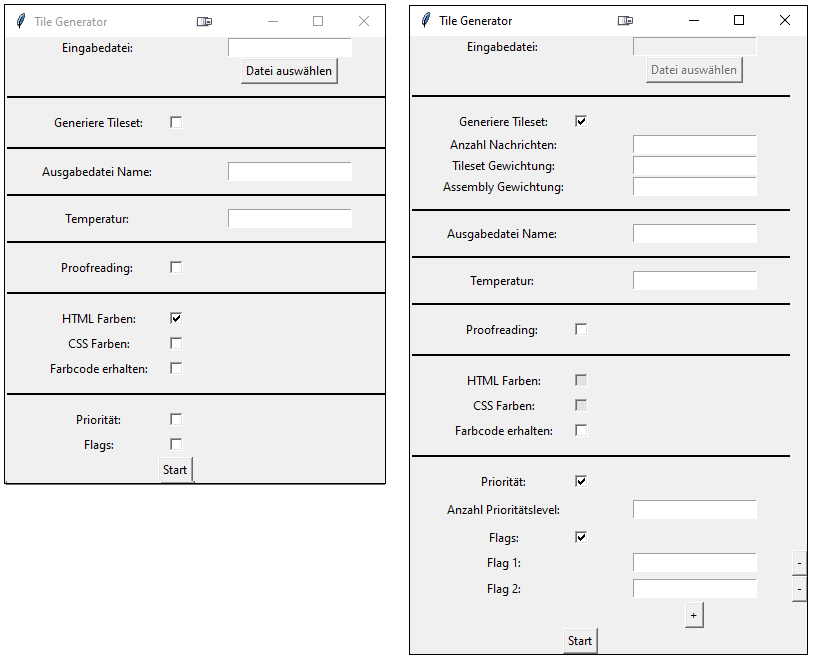
\includegraphics[width=\textwidth]{images/Tile-Generator.png}
    \caption[GUI Screenshot]{Darstellung des grafischen Interfaces des im Zuge dieser Arbeit entstandenen Skripts. Links ist dabei das Fenster ohne weitere Auswahl dargestellt. Rechts sind alle zusätzlichen Eingaben und Optionen gezeigt, die beim Auswählen aller Checkboxen hinzugefügt werden.}
    \label{fig:gui}
\end{figure}

Von Oben nach Unten sind die Einstellungsoptionen des Skripts wie folgt: Die Auswahl einer Eingabedatei fällt auf den Fall, dass ein in NetTAS erstelltes Tileset verwendet wird. Die entsprechende Datei muss über einen Datenexplorer ausgewählt werden. Wird die Checkbox \emph{Generiere Tileset} darunter ausgewählt, so öffnen sich drei Eingabefelder und eine Checkbox. Button und Eingabefeld der Eingabedatei werden dabei deaktiviert. 

In den neuen Eingabefeldern können die folgenden drei Parameter festgelegt werden: die Anzahl der Nachrichten, die durch das Tileset darstellbar sein sollen, die Gewichtung des Tileset und die Gewichtung der Self-Assembly. Alle drei Eingaben müssen ganze Zahlen beinhalten und sollte eine andere Eingabe getätigt werden, so wird diese mit einer Fehlernachricht abgefangen. Die Gewichtung von Tileset und Assembly ist relativ. Das bedeutet, dass eine Eingabe von eins in der Tileset Gewichtung und einer zehn in der Gewichtung der Assembly äquivalent zu einer Eingabe von zehn in der Tileset Gewichtung zu einer 100 in der Gewichtung der Assembly ist. Durch Aktivieren der Checkbox mit der Beschriftung \emph{Prüfsumme erstellen} wird die Prüfsummenbildung für das generierte Tileset aktiviert.

Unter dem Abschnitt zur Generierung von Tilesets findet sich das Eingabefeld der Ausgabedatei. Darin muss der Name der Datei angegeben werden. Ein \texttt{.json} am Ende des Namens ist nicht notwendig. Namen mit anderen Dateiendungen oder ohne Dateiendung werden erkannt und durch ein \texttt{.json} erweitert. Die Ausgabedatei wird immer an der gleichen Stelle im Verzeichnis wie das Skript abgespeichert.

Unter dem Eingabefeld für den Namen der Ausgabedatei ist ein weiteres Eingabefeld zu finden. Dieses dient zur Angabe der Temperatur. Auch hier kann erneut nur eine ganze Zahl angegeben werden, andere Eingaben führen zu einer Fehlermeldung. Darunter findet sich eine Checkbox mit der Beschriftung \emph{Proofreading}. Wird diese Checkbox ausgewählt, so wird auf das finale Tileset \emph{Snaked-Proofreading} angewendet.

Unter dieser Checkbox finden sich drei weitere Checkboxen. Die oberen beiden sind gegenseitig ausschließend, sodass immer nur eine aktiv sein kann. Mit ihnen kann anhand der Beschriftung angegeben werden, ob \emph{HTML Farben} oder \emph{CSS-Farben} als Farbkodierung verwendet werden. Im Fall einer Eingabedatei muss die Checkbox dem gewählten Farbschema aus dem Eingabetileset entsprechen. Ansonsten erscheint eine Fehlermeldung und das Skript kann nicht ausgeführt werden. Wird ein Tileset generiert, so sind diese beiden Checkboxen ausgegraut und nicht auswählbar, da sie keine Relevanz besitzen. Das generierte Tileset hat immer die Höhe eins und die einzige Farbkodierung ist ein Seed-Tile, das in HTML-Farbcode nach Tabelle~\ref{tab:farbkodierung} dargestellt wird. Die restlichen Tiles sind weiß codiert. Die dritte Checkbox, bezeichnet als \emph{Farbcode erhalten}, steuert die Farbkodierung des Ergebnistilesets. Ist diese Option aktiviert, bleibt die Farbkodierung im generierten Tileset bestehen. Andernfalls wird die Farbkodierung entfernt und nur die Tiles, die den Frame des Moleküls darstellen, werden in der Farbe Ozeangrün hervorgehoben, um eine bessere Übersicht zu gewährleisten. Es sei angemerkt, dass Ozeangrün die Primärfarbe des Farbschemas der Universität Lübeck ist.

Unter den drei Checkboxen für die Farbkodierung, finden sich zwei weitere Checkboxen. Die erste Checkbox für die \emph{Priorität} kann ausgewählt werden, wenn für das gegebene Tileset Prioritätstiles benötigt werden. Der genaue Ablauf wird in den folgenden Absätzen genauer betrachtet. Ist die Checkbox ausgewählt, öffnet sich ein Eingabefeld, in welchen eine ganze Zahl angegeben werden muss, um so anzugeben, wie viele Prioritätslevel es gibt. Die andere Checkbox mit dem Bezeichner \emph{Flags} öffnet beim Auswählen einen Button, der mit \glqq +\grqq~ bezeichnet wird. Durch diesen Button können beliebig viele Flags erzeugt werden, indem die dabei erscheinenden Eingabefelder mit Namen für die Tiles ausgefüllt werden. Mit dem rechts erscheinenden Button, gekennzeichnet durch ein \glqq -\grqq, kann eine falsch erstellte Flag wieder gelöscht werden. Ganz unten befindet sich der \emph{Start}-Button, der das Skript mit den oben angegeben Optionen ausführt. Danach öffnet sich der Datenexplorer an der Stelle, an der die Ausgabedatei gespeichert wird.

\section{Anforderungen für das korrekte Ausführen des Skripts}

Mit allen erforderlichen Optionen und Eingabe, können im Weiteren die Anforderungen für in NetTAS erstellte Tilesets festgelegt werden, die erfüllt werden müssen, damit das Skript funktioniert. Danach sollen auch die Anforderungen angegeben werden, die eingehalten werden sollten, um mögliche Fehler zu vermeiden. Zuletzt sollen die Anforderungen vorgestellt werden, die erfüllt werden können, um ein korrektes Skriptverhalten zu sichern.

\subsection{Notwendige Anforderungen an Tilesets}

In dieser Sektion werden die Anforderungen präsentiert, die für eine korrekte Funktionsweise des Skripts berücksichtigt werden müssen. Ein Nichtbefolgen dieser Anforderungen führt fast immer zu Fehlern. Einige dieser Fehler werden durch das Skript mit einer Fehlermeldung identifiziert, während andere zu fehlerhaften Tilesets führen können. Die erste Anforderung, das Einhalten des Farbcodes, wurde bereits bei der Beschreibung des grafischen Interfaces gegeben.

Die zweite Anforderung betrifft die Ausrichtung des Moleküls im Tileset. Das Molekül muss so konstruiert werden, dass es mit der Seed-Assembly rechts beginnt und nach links wächst. Beginnt die Seed-Assembly hingegen rechts, oben oder unten und das Molekül wächst dann in eine andere Richtung (links, unten oder oben), kann dies im Skript zu schwerwiegenden Fehlern führen.

Ein weiterer essentieller Aspekt ist die klare Definition einer Wachstumsfront an einer Molekülseite. Zur Verdeutlichung dieser Anforderung sind in Abbildung~\ref{fig:negativbsp_konstruktion} Negativbeispiele gezeigt. Es ist wichtig zu betonen, dass diese spezifische Anforderung primär im Kontext des Proofreadings relevant ist. Bei Konstruktionen ohne Proofreading könnten solche Strukturen problemlos sein. Bei Anwendung des Proofreadings ist es jedoch von zentraler Bedeutung, dass das verwendete Tileset konform mit den Wachstumsvorgaben ist. Im Proofreading-Verfahren beginnt das Wachstum stets in einem von vier festgelegten Tiles. Der Farbcode ermöglicht eine differenzierte Wachstumsdynamik in verschiedenen Molekülteilen, aber es muss stets eine konsistente Wachstumsfront beibehalten werden.

In Abbildung~\ref{fig:negativbsp_konstruktion} a) ist ein Beispiel für nicht-konformes Wachstum im Kontext des Proofreadings dargestellt. Bei Molekülen mit einer Höhe von mehr als einem Tile wird davon ausgegangen, dass das Wachstum vom Seed-Tile ausgeht. Für das in der Abbildung gezeigte Molekül wäre an der mit einem roten Kreis hervorgehobenen Position ein Kleber erforderlich.

In Abbildung~\ref{fig:negativbsp_konstruktion} b) wird ein weiteres Problem bei der Wachstumsfront dargestellt.
Für das Proofreading der zentralen Tiles bei Molekülen der Höhe drei ist es von Bedeutung, aus welcher Richtung das Wachstum erfolgt. Alle Tiles starten ihr Wachstum bei einem der vier Proofreadingtiles.
Um dies zu gewährleisten, muss eine der beiden Seiten so gebildet werden, dass sie ohne Verbindung eines zentralen Tiles auskommt. In dem dargestellten Beispiel erfordert dies das Hinzufügen von Klebern an den Stellen, die durch die blauen oder den roten Kreis markiert sind.

Das letzte Negativbeispiel ist in Abbildung~\ref{fig:negativbsp_konstruktion} c) zu sehen und ist mit dem Beispiel aus b) verbunden. In Molekülen der Höhe drei müssen die zentralen Tiles entweder von der Seed-Assembly, von der südlichen Grenze oder von der nördlichen Grenze startend wachsen. Ein Wachstum wie in c) wird durch das Skript nicht unterstützt, weshalb hier ein Kleber an einer der farbig markierten Stellen notwendig wäre.

\begin{figure}
    \centering
    \begin{tikzpicture}[scale=0.85]
        \node at (-0.4,1.7) {a)};
        \draw[fill=uzl_mediumblue_3] (0,0) rectangle (1,1);
        \draw[fill=black] (1,0.4) rectangle (1.2,0.6);
        \draw[fill=black] (2.2,0.4) rectangle (2.4,0.6);
        \draw[fill=black] (3.4,0.4) rectangle (3.6,0.6);
        \draw[fill=uzl_mediumblue_2] (1.2,0) rectangle (2.2,1);
        \draw[fill=uzl_mediumblue_2] (2.4,0) rectangle (3.4,1);
        \draw[fill=uzl_mediumblue_1] (3.6,0) rectangle (4.6,1);
        %
        \draw[fill=black] (0.4,1) rectangle (0.6,1.2);
        \draw[fill=black] (1.6,1) rectangle (1.8,1.2);
        \draw[fill=black] (2.8,1) rectangle (3,1.2);
        %
        \draw (0,1.2) rectangle (1,2.2);
        \draw[fill=black] (1,1.6) rectangle (1.2,1.8);
        \draw[fill=black] (2.2,1.6) rectangle (2.4,1.8);
        \draw[fill=black] (3.4,1.6) rectangle (3.6,1.8);
        \draw (1.2,1.2) rectangle (2.2,2.2);
        \draw (2.4,1.2) rectangle (3.4,2.2);
        \draw[fill=uzl_yellow_1] (3.6,1.2) rectangle (4.6,2.2);
        %
        \draw[fill=black] (0.4,2.2) rectangle (0.6,2.4);
        \draw[fill=black] (1.6,2.2) rectangle (1.8,2.4);
        \draw[fill=black] (2.8,2.2) rectangle (3,2.4);
        \draw[fill=black] (4,2.2) rectangle (4.2,2.4);
        %
        \draw[fill=uzl_red_3] (0,2.4) rectangle (1,3.4);
        \draw[fill=black] (1,2.8) rectangle (1.2,3);
        \draw[fill=black] (2.2,2.8) rectangle (2.4,3);
        \draw[fill=black] (3.4,2.8) rectangle (3.6,3);
        \draw[fill=uzl_red_2] (1.2,2.4) rectangle (2.2,3.4);
        \draw[fill=uzl_red_2] (2.4,2.4) rectangle (3.4,3.4);
        \draw[fill=uzl_red_1] (3.6,2.4) rectangle (4.6,3.4);
        %
        \draw[red, thick] (4.1,1.1) circle (0.3cm);
        %
        %
        %
        %
        \node at (5.4,1.7) {b)};
        \draw[fill=uzl_mediumblue_3] (5.8,0) rectangle (6.8,1);
        \draw[fill=black] (6.8,0.4) rectangle (7,0.6);
        \draw[fill=black] (9.2,0.4) rectangle (9.4,0.6);
        \draw[fill=uzl_mediumblue_2] (7,0) rectangle (8,1);
        \draw[fill=uzl_mediumblue_2] (8.2,0) rectangle (9.2,1);
        \draw[fill=uzl_mediumblue_1] (9.4,0) rectangle (10.4,1);
        %
        \draw[fill=black] (6.2,1) rectangle (6.4,1.2);
        \draw[fill=black] (7.4,1) rectangle (7.6,1.2);
        \draw[fill=black] (8.6,1) rectangle (8.8,1.2);
        \draw[fill=black] (9.8,1) rectangle (10,1.2);
        %
        \draw (5.8,1.2) rectangle (6.8,2.2);
        \draw (7,1.2) rectangle (8,2.2);
        \draw (8.2,1.2) rectangle (9.2,2.2);
        \draw[fill=uzl_yellow_1] (9.4,1.2) rectangle (10.4,2.2);
        %
        \draw[fill=black] (6.2,2.2) rectangle (6.4,2.4);
        \draw[fill=black] (7.4,2.2) rectangle (7.6,2.4);
        \draw[fill=black] (8.6,2.2) rectangle (8.8,2.4);
        \draw[fill=black] (9.8,2.2) rectangle (10,2.4);
        %
        \draw[fill=uzl_red_3] (5.8,2.4) rectangle (6.8,3.4);
        \draw[fill=black] (8,2.8) rectangle (8.2,3);
        \draw[fill=uzl_red_2] (7,2.4) rectangle (8,3.4);
        \draw[fill=uzl_red_2] (8.2,2.4) rectangle (9.2,3.4);
        \draw[fill=uzl_red_1] (9.4,2.4) rectangle (10.4,3.4);
        %
        \draw[blue, thick] (9.3,2.9) circle (0.3cm);
        \draw[blue, thick] (6.9,2.9) circle (0.3cm);
        \draw[red, thick] (8.1,0.5) circle (0.3cm);
        %
        %
        %
        %
        \node at (11.2,1.7) {c)};
        \draw[fill=uzl_mediumblue_3] (11.6,0) rectangle (12.6,1);
        \draw[fill=black] (12.6,0.4) rectangle (12.8,0.6);
        \draw[fill=black] (13.8,0.4) rectangle (14,0.6);
        \draw[fill=black] (15,0.4) rectangle (15.2,0.6);
        \draw[fill=uzl_mediumblue_2] (12.8,0) rectangle (13.8,1);
        \draw[fill=uzl_mediumblue_2] (14,0) rectangle (15,1);
        \draw[fill=uzl_mediumblue_1] (15.2,0) rectangle (16.2,1);
        %
        \draw[fill=black] (12,1) rectangle (12.2,1.2);
        \draw[fill=black] (13.2,1) rectangle (13.4,1.2);
        \draw[fill=black] (15.6,1) rectangle (15.8,1.2);
        %
        \draw (11.6,1.2) rectangle (12.6,2.2);
        \draw[fill=black] (12.6,1.6) rectangle (12.8,1.8);
        \draw[fill=black] (13.8,1.6) rectangle (14,1.8);
        \draw (12.8,1.2) rectangle (13.8,2.2);
        \draw (14,1.2) rectangle (15,2.2);
        \draw[fill=uzl_yellow_1] (15.2,1.2) rectangle (16.2,2.2);
        %
        \draw[fill=black] (12,2.2) rectangle (12.2,2.4);
        \draw[fill=black] (13.2,2.2) rectangle (13.4,2.4);
        \draw[fill=black] (15.6,2.2) rectangle (15.8,2.4);
        %
        \draw[fill=uzl_red_3] (11.6,2.4) rectangle (12.6,3.4);
        \draw[fill=black] (12.6,2.8) rectangle (12.8,3);
        \draw[fill=black] (13.8,2.8) rectangle (14,3);
        \draw[fill=black] (15,2.8) rectangle (15.2,3);
        \draw[fill=uzl_red_2] (12.8,2.4) rectangle (13.8,3.4);
        \draw[fill=uzl_red_2] (14,2.4) rectangle (15,3.4);
        \draw[fill=uzl_red_1] (15.2,2.4) rectangle (16.2,3.4);
        %
        \draw[blue, thick] (14.5,2.3) circle (0.3cm);
        \draw[green, thick] (15.1,1.7) circle (0.3cm);
        \draw[red, thick] (14.5,1.1) circle (0.3cm);
    \end{tikzpicture}
    \caption[Negativbeispiele für die Konstruktion durch das Skript]{Drei Beispiele von Tile-Assemblies, die im Skript zu Fehlern führen. Fehlen die Kleber zwischen Seedtiles und ihren nördlichen und südlichen Nachbarn, kann im Skript beim Proofreading keine korrekte Wachstumsrichtung gefunden werden. Dies ist in a) dargestellt. Auch muss entweder die nördliche Grenze oder die südliche Grenze des Moleküls durchgängig verbunden sein, da im Skript eine der beiden Seiten als Wachstumsfront definiert wird und das nicht mitten im Molekül wechseln kann. Das ist in b) zu sehen. Auch müssen alle zentralen Tiles (hier weiß codiert) von Norden, Süden oder Osten wachsen. Ein Wachstum von Westen bei zentralen Tiles ist nicht vorgesehen.}
    \label{fig:negativbsp_konstruktion}
\end{figure}

Die vierte Anforderung besagt, dass das ausgewählte Tileset für die gewählte Temperatur korrekt konstruiert sein muss. Das Skript selbst nimmt keine Korrekturen an fehlerhaften Verbindungen oder Tiles vor.

Die fünfte und abschließende Anforderung bezieht sich auf die Konsistenz von Kleberbezeichnern und Kleberstärken.Ein Tile darf auf keiner Seite einen Kleberbezeichner aufweisen, wenn dieser keine zugehörige Kleberstärke hat. Umgekehrt sollte keine Seite eines Tiles eine Kleberstärke > 0 besitzen, ohne durch einen entsprechenden Kleberbezeichner gekennzeichnet zu sein. Im Skript werden beide Werte zur Herleitung des jeweils anderen genutzt.

\subsection{Empfehlenswerte Anforderungen an Tilesets}

Im Folgenden werden empfohlene Anforderungen vorgestellt, die, obwohl nicht zwingend erforderlich, dazu beitragen, potenzielle Fehlerquellen zu minimieren. Es sollte betont werden, dass ein Nichteinhalten dieser Anforderungen nicht notwendigerweise zu Problemen führt. 

Ein zentrales Element dieser Empfehlungen ist die Notwendigkeit eines eindeutigen Bezeichners für jedes Tile. Dies ist insbesondere relevant, da beim Erstellen von Flag-, Prioritäts- und Snaked-Proofreading Tiles zusätzliche Kleberbezeichner benötigt werden. Diese werden durch Konkatenation des Tilebezeichners mit Zeichen aus einer nachfolgend dargestellten Liste generiert. Da so einige Kleberbezeichner automatisch entstehen, muss darauf geachtet werden, dass erstellte Kleberbezeichner nicht gleich heißen.
Im Skript wird für die erste Stelle der drei inneren Kleber eine kleingeschriebene Version des Tilebezeichners verwendet und danach mit drei Zeichen aus folgender Liste konkateniert:
\begin{align*}
    [0,1,\dots,8,9,a,b,\dots,y,z,aa,ab,\dots,zy,zz]
\end{align*}
Um zu verdeutlichen, wie die Kleberbezeichner generiert werden, wird das folgende Beispiel betrachtet:
\begin{description}
    \item[gegeben:]\hfill 
    \begin{itemize}
        \item vier Tiles mit dem Bezeichner $X$,
        \item ein Tile mit dem Bezeichner $Y$,
        \item zwei Tiles ohne Bezeichner.
    \end{itemize}
    \item[innere Bezeichnertripel:]\hfill
    \begin{itemize}
        \item~[$x0,x1,x2$],[$x3,x4,x5$],[$x6,x7,x8$],[$x9,xa,xb$],
        \item~[$y0,y1,y2$],
        \item~[$0,1,2$],[$3,4,5$].
    \end{itemize}
\end{description}

Dementsprechend muss beachtet werden, dass bei leeren Tilebezeichnern die generierten Kleberbezeichner einstellige Zahlen oder Buchstaben sind. Durch die Regeln der Self-Assembly kann es so beim automatischen Generieren von Kleberbezeichnern zu Wachstumsfehlern kommen. Wenn jedoch bei der Konstruktion des Tilesets in NetTAS darauf geachtet wird, muss dies keine Wachstumsfehler verursachen.

Damit verbunden sind allgemeine Regeln zur Kleberbezeichnung. Selbst wenn alle Tiles einen Bezeichner erhalten, sollte darauf geachtet werden, dass die genutzten Kleberbezeichner entweder einstellig und kleingeschrieben sind oder den folgenden Regeln entsprechen:

\begin{enumerate}
\item Bei Kleberbezeichnern mit einer Zeichenlänge von zwei oder drei darf das letzte Zeichen weder eine Zahl noch ein klein geschriebener Buchstabe sein.
\item Ein $<$ am Ende von Bezeichnern der Länge zwei kann zu Fehlern führen.
\item Kombinationen von $\{1,2\}$ am Anfang, beliebig vielen Zeichen in der Mitte und $\{F,P\}$ am Ende können von Flag- oder Prioritätstiles belegt sein.
\item Die Bezeichner $\sigma t, \sigma c$ und $\sigma b$ können belegt sein.
\item Großgeschriebene Buchstaben wie $\{A,B,\dots,Y,Z,AA,AB,\dots,ZY,ZZ\}$ werden vom Skript generiert und sollten daher nicht manuell vergeben werden.
\end{enumerate}

Während die Verwendung dieser Bezeichner nicht zwangsläufig Probleme verursacht, wird empfohlen, sie zu vermeiden, um potentiellen Fehlern vorzubeugen.

Insgesamt können durch die Zeichenmengen bis zu 237 gleich benannte Tiles unterschieden werden. Der Vollständigkeit halber muss trotzdem angemerkt werden, dass nicht mehr als 238 Mal der gleiche Tilebezeichner in einem Tileset verwendet werden sollte. 
Auch sind die Farbcodes für Flag- und Prioritätstiles im Skript zugelassen und führen nicht zu einem Error, wenn sie verwendet werden. Doch sind diese Farben nicht dafür gedacht, importiert zu werden. Sie werden im Skript als \emph{white} gewertet und müssen so platziert werden, damit es zu keinen Fehlern kommt. Es ist empfehlenswert diese Farben im gegeben Tileset nicht zu verwenden.

\subsection{Vorschläge für Tilesets}

Zuletzt werden noch einige Leitideen gegeben, denen gefolgt werden kann. Die sicherste Variante ist es, ein Tileset zu generieren. Das funktioniert bei sinnvollen und korrekten Eingaben im grafischen Interface immer fehlerfrei. Wenn jedoch ein Tileset in NetTAS erstellt wird, dann können die folgenden zwei Regeln eingehalten werden, um Fehlern vorzubeugen: Die Temperatur sollte zwischen zwei und drei gewählt werden und Tilesets für Moleküle sollten den Formen aus den Beispielen in dieser Arbeit folgen. Diese wurden alle getestet und funktionieren fehlerfrei. In Abbildung~\ref{fig:molekuel_form} sind die Molekülformen für die Höhen drei (in a,b und c), zwei ( in d und e)  und eins (in c) gegeben. All diese Strukturen wurden ausreichend getestet und funktionieren im Skript. Durch die Pfeile ist das Wachstum im Proofreading verbildlicht. Die grünen Pfeile repräsentieren die minimalen Kleberverbindungen zwischen den Molekülen. Die schwarz gestrichelten Pfeile hingegen symbolisieren zusätzliche, optionale Verbindungen. Während sie nicht zwingend für die Bildung eines Moleküls dieser Form benötigt werden, können sie dennoch notwendig sein, um eine entsprechende Berechnung in der Self-Assembly zu ermöglichen.

\begin{figure}
    \centering
    \begin{tikzpicture}[scale=0.8]
        \node at (-0.5,5.7) {a)};
        %
        \draw[fill=uzl_mediumblue_3] (0,4) rectangle (1,5);
        \draw[fill=uzl_mediumblue_2] (1.2,4) rectangle (2.2,5);
        \draw[fill=uzl_mediumblue_2] (2.4,4) rectangle (3.4,5);
        \draw[fill=uzl_mediumblue_1] (3.6,4) rectangle (4.6,5);
        %
        \draw (0,5.2) rectangle (1,6.2);
        \draw (1.2,5.2) rectangle (2.2,6.2);
        \draw (2.4,5.2) rectangle (3.4,6.2);
        \draw[fill=uzl_yellow_1] (3.6,5.2) rectangle (4.6,6.2);
        %
        \draw[fill=uzl_red_3] (0,6.4) rectangle (1,7.4);
        \draw[fill=uzl_red_2] (1.2,6.4) rectangle (2.2,7.4);
        \draw[fill=uzl_red_2] (2.4,6.4) rectangle (3.4,7.4);
        \draw[fill=uzl_red_1] (3.6,6.4) rectangle (4.6,7.4);
        %
        %
        \draw[green, thick, ->] (4.1,5.6) -- (4.1,4.5) -- (1.8,4.5);
        \draw[green, thick, ->] (4.1,5.8) -- (4.1,6.9) -- (1.8,6.9);
        \draw[green, thick, ->] (1.7,4.6) -- (1.7,5.6);
        \draw[green, thick, ->] (2.9,4.6) -- (2.9,5.6);
        \draw[green, thick, ->] (1.6,5.7) -- (0.5,5.7) -- (0.5,6.8);
        \draw[green, thick, ->] (0.5,5.7) -- (0.5,4.6);
        \draw[dashed, thick, ->] (1.6,4.5) -- (0.6,4.5);
        \draw[dashed, thick, ->] (1.6,6.9) -- (0.6,6.9);
        \draw[dashed, thick, ->] (1.7,6.8) -- (1.7,5.8);
        \draw[dashed, thick, ->] (2.9,6.8) -- (2.9,5.8);
        \draw[dashed, thick, ->] (4,5.7) -- (1.8,5.7);
        %
        %
        \node at (5.5,5.7) {b)};
        %
        \draw[fill=uzl_mediumblue_3] (6,4) rectangle (7,5);
        \draw[fill=uzl_mediumblue_2] (7.2,4) rectangle (8.2,5);
        \draw[fill=uzl_mediumblue_2] (8.4,4) rectangle (9.4,5);
        \draw[fill=uzl_mediumblue_1] (9.6,4) rectangle (10.6,5);
        %
        \draw (6,5.2) rectangle (7,6.2);
        \draw (7.2,5.2) rectangle (8.2,6.2);
        \draw (8.4,5.2) rectangle (9.4,6.2);
        \draw[fill=uzl_yellow_1] (9.6,5.2) rectangle (10.6,6.2);
        %
        \draw[fill=uzl_red_3] (6,6.4) rectangle (7,7.4);
        \draw[fill=uzl_red_2] (7.2,6.4) rectangle (8.2,7.4);
        \draw[fill=uzl_red_2] (8.4,6.4) rectangle (9.4,7.4);
        \draw[fill=uzl_red_1] (9.6,6.4) rectangle (10.6,7.4);
        %
        %
        \draw[green, thick, ->] (10.1,5.6) -- (10.1,4.5) -- (7.8,4.5);
        \draw[green, thick, ->] (10.1,5.8) -- (10.1,6.9) -- (7.8,6.9);
        \draw[dashed, thick, ->] (7.7,4.6) -- (7.7,5.6);
        \draw[dashed, thick, ->] (8.9,4.6) -- (8.9,5.6);
        \draw[green, thick, ->] (7.6,5.7) -- (6.5,5.7) -- (6.5,6.8);
        \draw[green, thick, ->] (6.5,5.7) -- (6.5,4.6);
        \draw[dashed, thick, ->] (7.6,4.5) -- (6.6,4.5);
        \draw[dashed, thick, ->] (7.6,6.9) -- (6.6,6.9);
        \draw[green, thick, ->] (7.7,6.8) -- (7.7,5.8);
        \draw[green, thick, ->] (8.9,6.8) -- (8.9,5.8);
        \draw[dashed, thick, ->] (10,5.7) -- (7.8,5.7);
        %
        %
        \node at (11.5,5.7) {c)};
        %
        \draw[fill=uzl_mediumblue_3] (12,4) rectangle (13,5);
        \draw[fill=uzl_mediumblue_2] (13.2,4) rectangle (14.2,5);
        \draw[fill=uzl_mediumblue_2] (14.4,4) rectangle (15.4,5);
        \draw[fill=uzl_mediumblue_1] (15.6,4) rectangle (16.6,5);
        %
        \draw (12,5.2) rectangle (13,6.2);
        \draw (13.2,5.2) rectangle (14.2,6.2);
        \draw (14.4,5.2) rectangle (15.4,6.2);
        \draw[fill=uzl_yellow_1] (15.6,5.2) rectangle (16.6,6.2);
        %
        \draw[fill=uzl_red_3] (12,6.4) rectangle (13,7.4);
        \draw[fill=uzl_red_2] (13.2,6.4) rectangle (14.2,7.4);
        \draw[fill=uzl_red_2] (14.4,6.4) rectangle (15.4,7.4);
        \draw[fill=uzl_red_1] (15.6,6.4) rectangle (16.6,7.4);
        %
        %
        \draw[green, thick, ->] (16.1,5.6) -- (16.1,4.5) -- (13.8,4.5);
        \draw[green, thick, ->] (16.1,5.8) -- (16.1,6.9) -- (13.8,6.9);
        \draw[dashed, thick, ->] (13.7,4.6) -- (13.7,5.6);
        \draw[dashed, thick, ->] (14.9,4.6) -- (14.9,5.6);
        \draw[green, thick, ->] (13.6,5.7) -- (12.5,5.7) -- (12.5,6.8);
        \draw[green, thick, ->] (12.5,5.7) -- (12.5,4.6);
        \draw[dashed, thick, ->] (13.6,4.5) -- (12.6,4.5);
        \draw[dashed, thick, ->] (13.6,6.9) -- (12.6,6.9);
        \draw[dashed, thick, ->] (13.7,6.8) -- (13.7,5.8);
        \draw[dashed, thick, ->] (14.9,6.8) -- (14.9,5.8);
        \draw[green, thick, ->] (16,5.7) -- (13.8,5.7);
        %
        %
        \node at (2.5,2.1) {d)};
        %
        \draw[fill=uzl_mediumblue_3] (3,1.2) rectangle (4,2.2);
        \draw[fill=uzl_mediumblue_2] (4.2,1.2) rectangle (5.2,2.2);
        \draw[fill=uzl_mediumblue_2] (5.4,1.2) rectangle (6.4,2.2);
        \draw[fill=uzl_mediumblue_1] (6.6,1.2) rectangle (7.6,2.2);
        %
        \draw (3,2.4) rectangle (4,3.4);
        \draw (4.2,2.4) rectangle (5.2,3.4);
        \draw (5.4,2.4) rectangle (6.4,3.4);
        \draw[fill=uzl_yellow_1] (6.6,2.4) rectangle (7.6,3.4);
        %
        %
        \draw[green, thick, ->] (7.1,2.8) -- (7.1,1.7) -- (4.8,1.7);
        \draw[green, thick, ->] (4.7,1.8) -- (4.7, 2.9) -- (3.5,2.9) -- (3.5,1.7);
        \draw[green, thick, ->] (5.9,1.7) -- (5.9,2.8);
        \draw[dashed, thick, ->] (7,2.9) -- (4.8,2.9);
        \draw[dashed, thick, ->] (4.6,1.7) -- (3.6,1.7);
        %
        %
        \node at (8.5,2.1) {e)};
        %
        \draw[fill=uzl_mediumblue_3] (9,1.2) rectangle (10,2.2);
        \draw[fill=uzl_mediumblue_2] (10.2,1.2) rectangle (11.2,2.2);
        \draw[fill=uzl_mediumblue_2] (11.4,1.2) rectangle (12.4,2.2);
        \draw[fill=uzl_mediumblue_1] (12.6,1.2) rectangle (13.6,2.2);
        %
        \draw (9,2.4) rectangle (10,3.4);
        \draw (10.2,2.4) rectangle (11.2,3.4);
        \draw (11.4,2.4) rectangle (12.4,3.4);
        \draw[fill=uzl_yellow_1] (12.6,2.4) rectangle (13.6,3.4);
        %
        %
        \draw[green, thick, ->] (13.1,2.8) -- (13.1,1.7) -- (10.8,1.7);
        \draw[green, thick, ->] (13, 2.9) -- (9.5,2.9) -- (9.5,1.7);
        \draw[dashed, thick, ->] (10.7,1.8) -- (10.7, 2.8);
        \draw[dashed, thick, ->] (11.9,1.7) -- (11.9,2.8);
        \draw[dashed, thick, ->] (10.6,1.7) -- (9.6,1.7);
        %
        %
        \node at (5.5,0) {f)};
        %
        \draw (6,-0.5) rectangle (7,0.5);
        \draw (7.2,-0.5) rectangle (8.2,0.5);
        \draw (8.4,-0.5) rectangle (9.4,0.5);
        \draw[fill=uzl_yellow_1] (9.6,-0.5) rectangle (10.6,0.5);
        %
        %
        \draw[green, thick, ->] (10.1,0) -- (6.6,0);
    \end{tikzpicture}
    \caption[Empfohlene Molekülformen]{Darstellung von verschiedenen Molekülformen, die empfohlen werden, um die korrekte Ausführung des Skripts zu gewährleisten. Die grünen Pfeile stellen dabei die minimal benötigten Kleber dar, die schwarz gestrichelten Pfeile sind nicht zwingend notwendig, könnten aber benötigt werden, wenn es die Logik der Assembly verlangt. a), b) und c) sind dabei verschiedene Möglichkeiten für Moleküle der Höhe drei. d) und e) sind die zwei möglichen Wachstumsrichtungen für Moleküle der Höhe zwei und f) stellt die eine triviale Wachstumsrichtung für Moleküle der Höhe eins dar.}
    \label{fig:molekuel_form}
\end{figure}

\section{Ablauf des Skripts}

Es wurden die Voraussetzungen vorgestellt, um möglichst fehlerfrei den Start-Button im grafischen Interface des Skripts drücken zu können. Damit kann im Folgenden genauer darauf eingegangen werden, was im Skript passiert, nachdem der Start-Button gedrückt wird. 

Wenn das Skript mit einer beliebigen Eingabe ausgeführt wird, erfolgt zunächst eine Prüfung der Eingabe. Dabei wird ermittelt, welche Checkboxen aktiviert wurden. Anschließend werden die zugehörigen Eingabefelder kontrolliert. So wird beispielsweise überprüft, ob die Eingabefelder von Temperatur, Nachrichtenanzahl, Tileset/Assembly Gewichtung und Priorität Zahlen sind. Für Flags, Eingabedatei und Ausgabedatei wird überprüft, ob sie nicht leer sind. Nur wenn alle Checks positiv sind, wird die Eingabe in die Main-Funktion übergeben, um dort das finale Tileset zu erstellen. Die Main-Funktion gibt das Tileset im \texttt{\_tiles} Dictionary zurück, wodurch dieses ohne weitere Änderungen in die Ausgabedatei geschrieben werden kann. Es erscheint eine Bestätigungsnachricht, dass das Skript erfolgreich ausgeführt wurde und der Datenexplorer öffnet sich am Speicherort der Ausgabedatei.

Für eine vollständig korrekte Ausführung muss noch betrachtet werden, was in der Main-Funktion passiert. Dies kann durch folgenden Pseudocode beschrieben werden: 
\begin{lstlisting}[language=python, caption={[Pseudocode der Main-Funktion des Skripts]{Pseudocode der Main-Funktion des Skripts. Es wird je nach Input eine Menge von Tiles erstellt, die für die Ausgabe vorbereitet werden. Dabei werden Informationen gesammelt, die im Code genutzt werden, um ein korrekt funktionierendes Tileset zu garantieren. Wurden in der GUI bestimmte Checkboxen aktiviert, so werden dementsprechend Flag-, Prioritäts- und Proofreadingtiles generiert.}}, label=lst:main]
def main(data, input)      
    new_tiles = []
    gatherinfo(data)
    if flags in input:
        data.add(flags)
    if priorities in input:
        data.add(priorities)
    sort(data, colorcode aus input)
    if proofreading in input:
        new_tiles = snakedproofreading(data)
    else:
        new_tiles = data 
    if not color_kept in input: 
        change_colors(new_tiles)
    return {"_tiles": new_tiles}
\end{lstlisting}

Der Hauptfunktion muss das gegebene oder generierte Tileset übergeben werden, sowie die angegebene Systemtemperatur und die Booleans für die Checkboxen im grafischen Interface. Daraufhin werden Informationen aus dem gegebenen Tileset entnommen. Dabei wird geprüft, ob das Tileset nördlich und südlich der Seed-Assembly entsprechende Tiles besitzt. Des Weiteren erfolgt die Überprüfung, ob mögliche südliche oder nördliche Grenzen innere Kleber besitzen, über die das Wachstum im Proofreading für die inneren Tiles gestartet werden kann. Zusätzlich wird der linke Kleber der Seed-Assembly vermerkt, um sicherzustellen, dass er bei der Erstellung der Flag- und Prioritätstiles erhalten bleibt. Wenn helleblaue oder hellrote Tiles existieren, werden auch ihre linken Kleber gespeichert.

In dieser Arbeit wird immer wieder von der Generierung oder Erstellung von Tiles geredet. Dies geschieht immer in einer Liste und durch eine allgemeine Definition einer \emph{generate\_tile}-Funktion. Diese Funktion gibt ein einzelnes Tile zurück, das in korrekter Darstellung nach dem Programmcode \ref{lst:tileset_json} angegeben wird. Im Folgenden ist ein Ausschnitt aus dem Skript aus Anhang \ref{app:code} \marginnote{\qrcode[height=1cm]{https://github.com/Falkenheim/Tile-Generator}} dargestellt, der jedes Mal mit passenden Parametern verwendet wird, um ein Tile zu erstellen.

\begin{lstlisting}[language=python, caption={[Codeausschnitt der \texttt{generate\_tile}-Funktion]{Die zentrale Funktion des Skriptes, mit welcher ein einzelnes Tile generiert werden kann. In \texttt{label} wird der Tilebezeichner gespeichert, im \texttt{glues}-Array die nördlichen, östlichen, südlichen und westlichen Kleber mit Bezeichner und Stärke. Dabei liegen sie auch in dieser Reihenfolge vor. Zuletzt kann noch die Füllfarbe des Tiles angegeben werden.}}, label=lst:generate_tile]
# t = tile
# l = label
# s = strength
# c = color
def generate_tile(tl, l1, s1, l2, s2, l3, s3, l4, s4, c):
    return {
        "label": tl,
        "glues": [
            {"label": l1, "strength": s1},
            {"label": l2, "strength": s2},
            {"label": l3, "strength": s3},
            {"label": l4, "strength": s4},
        ],
        "color": c
    }
\end{lstlisting}

\section{Erstellung von Flag- und Prioritätstiles}

Wenn alle Informationen gesammelt sind, dann werden Flags und Prioritätstiles erstellt. Dies passiert nur, wenn die jeweilige Checkbox ausgewählt wurde und die Eingabefelder nicht leer sind. Für alle erstellten und benannten Flags werden Tiles erstellt. 

Die Menge an benötigten Tiles ist dabei abhängig von der Höhe der Self-Assembly. Das heißt, dass aus den gesammelten Informationen entnommen wird, ob ein Tile der Farbe \emph{salmon} oder \emph{skyblue} existiert.
Diese müssen bei Existenz von Flag- oder Prioritätstiles am westlichen Kleber angepasst werden. Sie erhalten einen neuen Kleberbezeichner $\sigma t$, $\sigma c$ und $\sigma b$ für \texttt{top}, \texttt{center} und \texttt{bottom} Kleber. Somit wird in der Self-Assembly verhindert, dass sich das Molekül bindet, ohne die Flag- und Prioritätstiles hinzuzufügen. 

Auch muss beim Erstellen der Flagtiles beachtet werden, dass je nachdem, wie viele Flagtiles oder Prioritätstiles vorhanden sind, die westlichen Kleber des generierten Tiles verändert werden können. Dies ist in Abbildung \ref{fig:flag_prio_glues} dargestellt. In a) wird nur ein Flagtile ohne weitere Flag- oder Prioritätstiles erstellt. Dadurch ist der westliche Kleber des Flagtiles so gewählt, dass sich das restliche Molekül hier binden kann.
Dies ist analog für ein einzelnes Prioritätstile ohne Flag Tiles. In b) wird ein Flag- und ein Prioritätstile hinzugefügt. Dadurch braucht es einen zusätzlichen eindeutigen inneren Kleber zwischen Flag- und Prioritätstile. Der Vorgang ist wiederum analog für zwei Flagtiles. In c) ist der letzte Fall dargestellt, in welchem zwei Flagtiles und ein Prioritätstile hinzugefügt werden. Dabei werden mehrere innere Kleber benötigt. Es werden immer drei Kleberbezeichner aus der Menge $\{A,B,C,\dots,AA,AB,AC,\dots,ZX,ZY,ZZ\}$ entnommen. Somit sind bis zu 234 Flag- oder Prioritätstiles nebeneinander möglich.

\begin{figure}
    \centering
    \begin{tikzpicture}
        \tileFlagPrioZeroB{-1}{2.4}
        \tileFlagPrioZeroM{-1}{1.2}
        \tileFlagPrioZeroY{-1}{0}
        %
        \tileFlagPrioZeroA{0.2}{2.4}
        \tileFlagPrioZeroSigma{0.2}{1.2}
        \tileFlagPrioZeroX{0.2}{0}
        \node[scale=3] at (1.7,1.2) {$\Rightarrow$};
        %
        %
        %
        \node at (3,5.2) {a)};
        \tileFlagPrioOneB{4}{6.4}
        \tileFlagPrioOneM{4}{5.2}
        \tileFlagPrioOneY{4}{4}
        %
        \tileFlagPrioOneFt{5.2}{6.4}
        \tileFlagPrioOneFc{5.2}{5.2}
        \tileFlagPrioOneFb{5.2}{4}
        %
        \tileFlagPrioOneA{6.4}{6.4}
        \tileFlagPrioOneSigma{6.4}{5.2}
        \tileFlagPrioOneX{6.4}{4}
        %
        %
        %
        \node at (3,1.2) {b)};
        \tileFlagPrioTwoB{4}{2.4}
        \tileFlagPrioTwoM{4}{1.2}
        \tileFlagPrioTwoY{4}{0}
        %
        \tileFlagPrioTwoOneA{5.2}{2.4}
        \tileFlagPrioTwoOneB{5.2}{1.2}
        \tileFlagPrioTwoOneC{5.2}{0}
        %
        \tileFlagPrioTwoFt{6.4}{2.4}
        \tileFlagPrioTwoFc{6.4}{1.2}
        \tileFlagPrioTwoFb{6.4}{0}
        %
        \tileFlagPrioTwoA{7.6}{2.4}
        \tileFlagPrioTwoSigma{7.6}{1.2}
        \tileFlagPrioTwoX{7.6}{0}
        %
        %
        %
        \node at (3,-2.8) {c)};
        \tileFlagPrioThreeB{4}{-1.6}
        \tileFlagPrioThreeM{4}{-2.8}
        \tileFlagPrioThreeY{4}{-4}
        %
        \tileFlagPrioThreeOneD{5.2}{-1.6}
        \tileFlagPrioThreeOneE{5.2}{-2.8}
        \tileFlagPrioThreeOneF{5.2}{-4}
        %
        \tileFlagPrioThreeGA{6.4}{-1.6}
        \tileFlagPrioThreeGB{6.4}{-2.8}
        \tileFlagPrioThreeGC{6.4}{-4}
        %
        \tileFlagPrioThreeFt{7.6}{-1.6}
        \tileFlagPrioThreeFc{7.6}{-2.8}
        \tileFlagPrioThreeFb{7.6}{-4}
        %
        \tileFlagPrioThreeA{8.8}{-1.6}
        \tileFlagPrioThreeSigma{8.8}{-2.8}
        \tileFlagPrioThreeX{8.8}{-4}
    \end{tikzpicture}
    \caption[Kleberverhalten beim Hinzufügen von Flag- und Prioritätstiles]{Darstellung des inneren Kleberverhaltens für Flag- und Prioritätstiles. Sowohl a), b) und c) stammen original aus dem linken Molekül. In a) wird ein einzelnes Flag Tile im Molekül hinzugefügt. Dabei muss nur der Kleber an den Tiles \texttt{$\sigma$, A} und \texttt{X} geändert werden. Die Flag Tiles können dann östlich dieser Bezeichner und westlich die alten Bezeichner erhalten, an welchen \texttt{B,M} und \text{Y} gebunden werden. In b) ist das innere Kleberverhalten dargestellt. Die Kleberbezeichner \texttt{A,B,C} werden verwendet, um die Flag- und Prioritätstiles zu verbinden. Die restliche Kleberbezeichner sind analog zu a) gesetzt. In c) wird gezeigt wie die inneren Kleber sich im Weiteren verhalten. Das Flagtile mit dem Bezeichner \texttt{G} hat so komplett eigene Kleberbezeichner. Die restlichen Bezeichner sind wieder analog zu b) und a). Auch ist anzumerken, dass keine Unterscheidung in der Konstruktionsweise von zwei Flagtiles zu einem Flagtile und einem Prioritätstile gemacht wird.}
    \label{fig:flag_prio_glues}
\end{figure}

Wie angedeutet ist die Erstellung von Prioritätstiles analog zu den Flagtiles. Dabei muss nur darauf geachtet werden, ob und wie viele Flagtiles existieren, um so die korrekten östlichen Kleber erstellen zu können. Die westlichen Kleber sind immer die Kleber, die das restliche Molekül binden.

Sind Flag- und Prioritätstiles erstellt, wird zunächst das Tileset nach den Farben der Tiles sortiert. Dies wird zum einen aus Gründen der Übersicht vorgenommen, zum anderen, um sicherzustellen, dass die Seed-Assembly an erster Stelle steht. Denn so wird die Seed-Assembly in NetTAS festgelegt. Auch wird diese Sortierung bei der Anwendung von Snaked Proofreading verwendet. Wenn an dieser Stelle jedoch kein Proofreading vorgenommen werden soll, wird die Eingabemenge in die Liste \texttt{new\_tiles} übernommen. In dieser Liste wird dann noch die Farbkodierung entfernt, wenn nicht die entsprechende Checkbox ausgewählt wurde, durch die der Farbcode erhalten bleibt. Die Liste kann wie folgt zurückgegeben werden:
\begin{lstlisting}[language=python, caption={[Main-Funktion Rückgabe]{Die Rückgabe der Main-Funktion, die so erstellt wird, dass sie ohne Probleme in eine JSON-Ausgabedatei geschrieben werden kann.}}]
    return {"_tiles": new_tiles}
\end{lstlisting}

\section{Proofreading im Skript}

Wird jedoch Snaked-Proofreading auf das Tileset angewendet, dann wird die \texttt{new\_tiles}-Liste neu erstellt. Jedes Tile aus der sortierten Liste von Tiles in \texttt{data[\_tiles]} wird durch vier neue Tiles ersetzt. Dabei folgen die Tiles den Regeln des Snaked-Proofreadings aus dem Kapitel \ref{cha:grundlagen}, dargestellt in Abbildung \ref{fig:error_korrektur}. Diese vier Tiles müssen zusammen wieder die gleiche Information und Position des originalen Tiles beinhalten. 

Die so erstellten Tiles müssen dabei von einem der vier Tiles aus mit ihrem Wachstum starten. Je nach Position im Molekül kann dieses Wachstum mit einem anderen Tile starten. In Abbildung \ref{fig:snaked_wachstum} ist dies für alle farbcodierten Tiles dargestellt. 

\begin{figure}
    \centering
    \begin{tikzpicture}
        \node at (-0.8,6.6) {a)};
        \tileDirectionsLBtoRBOne{0}{7.2}{uzl_red_3}
        \tileDirectionsLBtoRBTwo{1.2}{7.2}{uzl_red_3}
        \tileDirectionsLBtoRBThree{0}{6}{uzl_red_3}
        \tileDirectionsLBtoRBFour{1.2}{6}{uzl_red_3}
        \draw[green, line width=2pt, ->] (1,6.2) -- (1,7) -- (0.2,7) -- (0.2,6.2);
        \draw[line width=2pt, ->] (2,6) -- (1.4,6);
        \draw[line width=2pt, ->] (1.2,5.2) -- (1.2,5.8);
        %
        \node at (2.2,6.6) {b)};
        \tileDirectionsLBtoRBOne{3}{7.2}{uzl_red_2}
        \tileDirectionsLBtoRBTwo{4.2}{7.2}{uzl_red_2}
        \tileDirectionsLBtoRBThree{3}{6}{uzl_red_2}
        \tileDirectionsLBtoRBFour{4.2}{6}{uzl_red_2}
        \draw[green, line width=2pt, ->] (4,6.2) -- (4,7) -- (3.2,7) -- (3.2,6.2);
        \draw[line width=2pt, ->] (5,6) -- (4.4,6);
        %
        \node at (5.2,6.6) {c)};
        \tileDirectionsLBtoRBOne{6}{7.2}{uzl_red_1}
        \tileDirectionsLBtoRBTwo{7.2}{7.2}{uzl_red_1}
        \tileDirectionsLBtoRBThree{6}{6}{uzl_red_1}
        \tileDirectionsLBtoRBFour{7.2}{6}{uzl_red_1}
        \draw[green, line width=2pt, ->] (7,6.2) -- (7,7) -- (6.2,7) -- (6.2,6.2);
        \draw[line width=2pt, ->] (7.2,5.2) -- (7.2,5.8);
        %
        \node at (-3.8,3.6) {d)};
        \tileDirectionsRTtoLTOne{-3}{4.2}{white}
        \tileDirectionsRTtoLTTwo{-1.8}{4.2}{white}
        \tileDirectionsRTtoLTThree{-3}{3}{white}
        \tileDirectionsRTtoLTFour{-1.8}{3}{white}
        \draw[green, line width=2pt, ->] (-2,4) -- (-2,3.2) -- (-2.8,3.2) -- (-2.8,4);
        \draw[line width=2pt, ->] (-1.8,5) -- (-1.8,4.4);
        %
        \node at (-0.8,3.6) {e)};
        \tileDirectionsLBtoRBOne{0}{4.2}{white}
        \tileDirectionsLBtoRBTwo{1.2}{4.2}{white}
        \tileDirectionsLBtoRBThree{0}{3}{white}
        \tileDirectionsLBtoRBFour{1.2}{3}{white}
        \draw[green, line width=2pt, ->] (1,3.2) -- (1,4) -- (0.2,4) -- (0.2,3.2);
        \draw[line width=2pt, ->] (2,3) -- (1.4,3);
        %
        \node at (2.2,3.6) {f)};
        \tileDirectionsLBtoRBOne{3}{4.2}{white}
        \tileDirectionsLBtoRBTwo{4.2}{4.2}{white}
        \tileDirectionsLBtoRBThree{3}{3}{white}
        \tileDirectionsLBtoRBFour{4.2}{3}{white}
        \draw[green, line width=2pt, ->] (4,3.2) -- (4,4) -- (3.2,4) -- (3.2,3.2);
        \draw[line width=2pt, ->] (4.2,2.2) -- (4.2,2.8);
        %
        \node at (5.2,3.6) {g)};
        \tileDirectionsLTtoLBOne{6}{4.2}
        \tileDirectionsLTtoLBTwo{7.2}{4.2}{white}
        \tileDirectionsLTtoLBFour{6}{3}{white}
        \tileDirectionsLTtoLBThree{7.2}{3}{white}
        \draw[green, line width=2pt, ->] (6.2,4) -- (7,4) -- (7,3.2) -- (6.2,3.2);
        %
        \node at (-0.8,0.6) {h)};
        \tileDirectionsRTtoLTOne{0}{1.2}{uzl_mediumblue_3}
        \tileDirectionsRTtoLTTwo{1.2}{1.2}{uzl_mediumblue_3}
        \tileDirectionsRTtoLTThree{0}{0}{uzl_mediumblue_3}
        \tileDirectionsRTtoLTFour{1.2}{0}{uzl_mediumblue_3}
        \draw[green, line width=2pt, ->] (1,1) -- (1,0.2) -- (0.2,0.2) -- (0.2,1);
        \draw[line width=2pt, ->] (2,1.2) -- (1.4,1.2);
        \draw[line width=2pt, ->] (1.2,2) -- (1.2,1.4);
        %
        \node at (2.2,0.6) {i)};
        \tileDirectionsRTtoLTOne{3}{1.2}{uzl_mediumblue_2}
        \tileDirectionsRTtoLTTwo{4.2}{1.2}{uzl_mediumblue_2}
        \tileDirectionsRTtoLTThree{3}{0}{uzl_mediumblue_2}
        \tileDirectionsRTtoLTFour{4.2}{0}{uzl_mediumblue_2}
        \draw[green, line width=2pt, ->] (4,1) -- (4,0.2) -- (3.2,0.2) -- (3.2,1);
        \draw[line width=2pt, ->] (5,1.2) -- (4.4,1.2);
        %
        \node at (5.2,0.6) {j)};
        \tileDirectionsRTtoLTOne{6}{1.2}{uzl_mediumblue_1}
        \tileDirectionsRTtoLTTwo{7.2}{1.2}{uzl_mediumblue_1}
        \tileDirectionsRTtoLTThree{6}{0}{uzl_mediumblue_1}
        \tileDirectionsRTtoLTFour{7.2}{0}{uzl_mediumblue_1}
        \draw[green, line width=2pt, ->] (7,1) -- (7,0.2) -- (6.2,0.2) -- (6.2,1);
        \draw[line width=2pt, ->] (7.2,2) -- (7.2,1.4);
    \end{tikzpicture}
    \caption[Wachstumrichtung für Tiles mit Snaked-Proofreading je nach Farbcode]{Darstellung der verschiedenen Wachstumsrichtungen von Tiles mit Snaked-Proofreading. Die Richtung ist durch die grünen Pfeile dargestellt, während durch die schwarzen Pfeile der Kleber angegeben wird, über welchen die Tiles beim Start gebunden werden. In g) ist die Seed-Assembly abgebildet, die nicht durch irgendwelche Kleberverbindungen gestartet wird. a), b) und c) sind die Tiles der nördlichen Grenze. h), i) und j) sind die Tiles der südlichen Grenze. Die drei Möglichkeiten in d), e) und f) für die weißen zentralen Tiles hängen von der Wachstumsfront während der Self-Assembly ab. d) wächst von Norden, e) von Osten und f) von Süden.}
    \label{fig:snaked_wachstum}
\end{figure}

Die Seed-Assembly wird als einziges Tile aus \glqq Nichts\grqq\, gebildet und ist dementsprechend an keine Regel gebunden, wenn es um die Wachstumsrichtung geht. Im Skript wurde diese Wachstumsrichtung gewählt, da in NetTAS, dass erste angegebene Tile als neues Seedtile dient. Da dies das linksobere Tile im Proofreading ist, kann somit die in Abbildung~\ref{fig:snaked_wachstum} g) dargestellte Richtung verwendet werden. 

Das hellrote Tile nördlich des Seedtiles muss das Wachstum mit dem Tile rechts unten starten. Der Grund dafür ist, dass sobald die beiden linken Tiles gebunden sind, die roten Tiles daneben gebunden werden können. Das soll aber erst passieren, wenn alle hellroten Tiles gebunden sind. Somit müssen zuerst die beiden rechten und danach die beiden linken Tiles gebunden werden.Die Kleber zwischen Seedtiles und den nördlichen Tiles müssen so angepasst werden, dass die rechten Tiles sich verbinden können. Gleichzeitig muss die Kleberstärke zwischen den linken Tiles so gewählt werden, dass sie sich erst dann verbinden, wenn alle drei anderen hellroten Tiles bereits gebunden sind. Die roten Tiles bilden die nördliche Grenze des Moleküls. Für sie gilt dieselbe Wachstumsrichtung. Nur der Kleber, über welchen das erste Tile gebunden wird, ist in diesem Fall östlich, statt südlich. Die dunkelroten Tiles repräsentieren die nördlichen Liganden. Es wird davon ausgegangen, dass sie sich erst dann bilden, wenn das gesamte Molekül korrekt verbunden ist. Dementsprechend wächst dieses zwar genau wie das hellrote und rote Tile, jedoch benötigt das erste Tile sowohl den östlichen als auch den südlichen Kleber dafür. Wenn ein Kleber auf einer Seite fehlt, muss der jeweils andere Kleber ausreichend stark sein, um die korrekte Bindung sicherzustellen.

Für die hellblauen, blauen und dunkelblauen Tiles ist dieses Verhalten analog zu den roten, nur dass das 
Wachstum mit den oberen Tiles starten muss, da die Tiles nach Süden wachsen müssen. Diese Tiles werden immer genau gleich gebildet. Jedoch hat nicht jedes durch Self-Assembly gebildete Molekül die gleiche Höhe. Dementsprechend müssen die inneren Tiles (weiß) immer abhängig von den Informationen über das Tileset gebildet werden. Auch kann es bei Molekülen der Höhe drei zu dem Problem kommen, dass sowohl der nördliche als auch der südliche Kleber benötigt wird, um ein Tile zu binden. Da beim Snaked-Proofreading jedoch zwei Tiles gebunden werden müssen, bevor südliche und nördliche Kleber verbunden werden, könnte Information verloren gehen. 

Das beschriebene Problem ist in Abbildung~\ref{fig:assembly_problem} aufgezeichnet. Dabei ist in a) eine Self-Assembly abgebildet, die bei Snaked-Proofreading ein Problem verursacht. Die inneren und weißen Tiles sind abhängig vom südlichen und nördlichen Tile.
Je nach nördlichem Kleber des Tiles \texttt{Y} und südlichem Kleber des Tiles \texttt{B} bindet sich ein anderes zentrales Tile. 

In b) kann das Problem erkannt werden, das entsteht, wenn auf solchen Tilesets Snaked-Proofreading angewendet wird. Das Wachstum der vier zentralen Tiles startet unten rechts. Damit sich dieses Tile bindet, muss der Kleber verstärkt werden. Dadurch kann sich jedoch ein falsches Tile binden, da noch keine Information des nördlichen Klebers verwendet wird. In b) bindet sich das Tile \texttt{0}. Damit gibt es im Tileset kein Tile mehr, das sich oben rechts binden kann. Die einzigen potenziellen Kandidaten sind über dem Molekül dargestellt. Die roten Markierungen weisen dabei darauf hin, weshalb auch diese Tiles nicht gebunden werden können.

Um das Problem zu lösen, muss wie in c) dargestellt, die Information des südlichen Klebers weitergegeben werden. Durch die Konkatenation mit dem Zeichen \glqq <\grqq\,wird sichergestellt, dass keine falsche Bindung entstehen kann. Die Information des südlichen Klebers wird dabei im inneren Kleber des Proofreadings mitgegeben. Somit kann sich das \glqq falsche\grqq\, Tile unten rechts bilden, ohne ein Problem zu verursachen. Das korrekte Tile bindet sich immer oben rechts.

\begin{figure}
    \centering
    \begin{tikzpicture}[scale=0.9]
        \node at (-6.2,3) {a)};
        \tileSPProblemBZero{-3.4}{6}
        \tileSPProblemYOne{-3.4}{0}
        \tileSPProblemOneBot{-5.2}{4.5}
        \tileSPProblemZero{-5.2}{3}
        \tileSPProblemTwo{-5.2}{1.5}
        %
        \tileSPProblemBOne{-3.4}{4.2}
        \tileSPProblemOneTop{-3.4}{3}
        \tileSPProblemYZero{-3.4}{1.8}
        %
        \tileSPProblemA{-2.2}{4.2}
        \tileSPProblemSigma{-2.2}{3}
        \tileSPProblemX{-2.2}{1.8}
        %
        %
        %
        \tileSPProblemSnakedZeroRT{0.3}{7.6}
        \draw[red, thick] (0.3,7.95) circle (0.2cm);
        \tileSPProblemSnakedOneTRT{1.8}{7.6}
        \draw[red, thick] (1.8,7.2) circle (0.2cm);
        \tileSPProblemSnakedTwoRT{3.3}{7.6}
        \draw[red, thick] (3.3,7.2) circle (0.2cm);
        %
        \node at (-1,3) {b)};
        \tileSPProblemSnakedBOneLT{0}{6}
        \tileSPProblemSnakedBOneRT{1.2}{6}
        \tileSPProblemSnakedBOneLB{0}{4.8}
        \tileSPProblemSnakedBOneRB{1.2}{4.8}
        %
        \tileSPProblemSnakedZeroRB{1.2}{2.4}
        %
        \tileSPProblemSnakedYZeroLT{0}{1.2}
        \tileSPProblemSnakedYZeroRT{1.2}{1.2}
        \tileSPProblemSnakedYZeroLB{0}{0}
        \tileSPProblemSnakedYZeroRB{1.2}{0}
        %
        \tileSPProblemSnakedALT{2.4}{6}
        \tileSPProblemSnakedART{3.6}{6}
        \tileSPProblemSnakedALB{2.4}{4.8}
        \tileSPProblemSnakedARB{3.6}{4.8}
        %
        \tileSPProblemSnakedSigmaLT{2.4}{3.6}
        \tileSPProblemSnakedSigmaRT{3.6}{3.6}
        \tileSPProblemSnakedSigmaLB{2.4}{2.4}
        \tileSPProblemSnakedSigmaRB{3.6}{2.4}
        %
        \tileSPProblemSnakedXLT{2.4}{1.2}
        \tileSPProblemSnakedXRT{3.6}{1.2}
        \tileSPProblemSnakedXLB{2.4}{0}
        \tileSPProblemSnakedXRB{3.6}{0}
        %
        %
        %
        %
        \node at (5,3) {c)};
        \tileSPProblemSnakedBOneLT{6}{6}
        \tileSPProblemSnakedBOneRT{7.2}{6}
        \tileSPProblemSnakedBOneLB{6}{4.8}
        \tileSPProblemSnakedBOneRB{7.2}{4.8}
        %
        \tileSPProblemSnakedOneTLT{6}{3.6}
        \tileSPProblemSnakedOneTRTFix{7.2}{3.6}
        \tileSPProblemSnakedOneTLB{6}{2.4}
        \tileSPProblemSnakedZeroRBFix{7.2}{2.4}
        %
        \tileSPProblemSnakedYZeroLT{6}{1.2}
        \tileSPProblemSnakedYZeroRT{7.2}{1.2}
        \tileSPProblemSnakedYZeroLB{6}{0}
        \tileSPProblemSnakedYZeroRB{7.2}{0}
        %
        \tileSPProblemSnakedALT{8.4}{6}
        \tileSPProblemSnakedART{9.6}{6}
        \tileSPProblemSnakedALB{8.4}{4.8}
        \tileSPProblemSnakedARB{9.6}{4.8}
        %
        \tileSPProblemSnakedSigmaLT{8.4}{3.6}
        \tileSPProblemSnakedSigmaRT{9.6}{3.6}
        \tileSPProblemSnakedSigmaLB{8.4}{2.4}
        \tileSPProblemSnakedSigmaRB{9.6}{2.4}
        %
        \tileSPProblemSnakedXLT{8.4}{1.2}
        \tileSPProblemSnakedXRT{9.6}{1.2}
        \tileSPProblemSnakedXLB{8.4}{0}
        \tileSPProblemSnakedXRB{9.6}{0}
    \end{tikzpicture}
    \caption[Snaked-Proofreading Problem für Moleküle der Höhe drei.]{Darstellung eines Problems von Snaked-Proofreading bei Molekülen der Höhe drei. In a) ist ein solches Molekül dargestellt. Abhängig vom südlichen Kleber von Tile \texttt{B} und dem nördlichen Kleber von Tile \texttt{Y} existieren die vier unterschiedlichen Tiles: \texttt{0,1,1} und \texttt{2}. Das Tile mit dem Bezeichner \texttt{1} gibt es dabei zweimal, da einmal die \texttt{1} von oben und einmal von unten geliefert wird. In b) kann das Problem bei dieser Self-Assembly erkannt werden. Da das zentrale Tile an der unteren rechten Seite das Wachstum starten muss, ist dort der Kleber stärker. So kann sich das Tile \texttt{0} binden und bei Temperatur drei halten. Jedoch müsste sich zur korrekten Bindung das Tile \texttt{1} binden. Es kann sich jedoch kein weiteres Tile binden, wie durch die rote Markierung darüber dargestellt wurde. Die Lösung für das Problem wird in c) dargestellt. Der Kleberbezeichner im Süden der Tiles (\texttt{0} bei Tiles \texttt{1} und \texttt{0} und \texttt{1} bei Tiles \texttt{1} und \texttt{2}) muss nach oben weitergegeben werden. Dafür wird der Bezeichner mit \texttt{<} konkateniert. Damit bindet sich rechtsoben das richtige Tile. Auch wenn unten \texttt{0} gebunden wird, kann durch die Weitergabe der \texttt{0} an den nördlichen Kleber, das korrekte Tile darüber gebunden werden.}
    \label{fig:assembly_problem}
\end{figure}

Wie in Abbildung~\ref{fig:snaked_wachstum} dargestellt wird, gibt es je nach Existenz der jeweiligen Tiles drei mögliche Wachstumsrichtungen. Gibt es blaue Tiles, die alle nördliche Kleber besitzen, so wachsen die inneren Tiles vom südlichen Kleber des rechten unteren Tiles aus. Das ist in Abbildung~\ref{fig:snaked_wachstum} f) dargestellt. Gibt es keine blauen Tiles im Tileset oder haben nicht alle blauen Tiles nördliche Kleber, so wird überprüft, ob es rote Tiles gibt. Falls alle diese Tiles einen südlichen Kleber besitzen, beginnt das Wachstum der inneren Tiles vom nördlichen Kleber aus, wobei mit dem rechtsoberen Tile gestartet wird. Das wird in Abbildung~\ref{fig:snaked_wachstum} d) gezeigt. Gilt keiner der beiden genannten Fälle, so müssen die inneren Tiles von der Seed-Assembly aus gebildet werden. Dabei wachsen die vier Tiles vom linken unteren Tile und dessen östlichem Kleber aus. Dies ist in Abbildung~\ref{fig:snaked_wachstum} e) zu sehen.

Damit sind alle Regeln für das Bilden der Tiles ausgelegt. So können die vier Tiles durch die entsprechenden Abfragen generiert werden. Für jedes Tile werden diese in der \texttt{new\_tiles}-Liste gesammelt. Sind alle Schritte und Funktionen aus Code~\ref{lst:main} durchlaufen, so wird der Inhalt in eine JSON-Datei geschrieben, die in NetTAS geladen und simuliert werden kann. 

In diesem Kapitel wurde die Konstruktion des Python-Skripts vorgestellt, mit welchem einige der Mechanismen aus dem vorherigen Kapitel in Tilesets implementiert werden. Auch wurde näher beschrieben, wie diese Mechanismen sinnvoll in Tilesets eingebaut werden können. Mit dem Skript und der Vorstellung dieser Mechanismen können im Weiteren Simulationen durchgeführt und die Ergebnisse evaluiert werden.